\documentclass{beamer}


\usepackage{amsmath}
\usepackage[style=alphabetic,url=true]{biblatex}
\usepackage{environ}
\usepackage{geometry}
\usepackage{graphicx}
\usepackage{tikz}
\usepackage[T2A]{fontenc}
\usepackage[utf8]{inputenc}
\usepackage[cache=false]{minted}
\usepackage{amsmath}
\usepackage{amsfonts}
\usepackage{amssymb}
\usepackage{calrsfs}
\usepackage{animate}
\usepackage{xmpmulti}


% \usetheme{Bergen}

\usecolortheme{beaver}

\setbeamertemplate{itemize item}[circle]
\setbeamertemplate{itemize subitem}{--}
\addtobeamertemplate{navigation symbols}{}{
  \usebeamerfont{footline}%
  \usebeamercolor[fg]{footline}%
  \hspace{1em}%
  \insertframenumber/\inserttotalframenumber
}
\graphicspath{ {./graphics/} }
\setminted[Python]{
  fontsize=\tiny
}
\BeforeBeginEnvironment{minted}{\medskip}
\AfterEndEnvironment{minted}{\medskip}
\usetikzlibrary{matrix}
\tikzset{
  stack/.style={
    matrix of nodes,
    nodes={
      fill=lightgray,draw,text=black,font=\sffamily\bfseries,
      text height=11pt,text depth=3pt,baseline=center, minimum width=1cm
    },
    column sep=-\pgflinewidth/2
  }
}

\title{
  Bitcoin and Cryptocurrency Technologies \\
  Lecture 6: Bitcoin Network
}

\author{Yuri Zhykin}
\date{Mar 29, 2021}

\begin{document}

\frame{\titlepage}

\begin{frame}
  \frametitle{Peer-to-Peer Networks 1/2}
  \begin{itemize}
  \item \textbf{Peer-to-peer} (\textbf{P2P}) \textbf{networking} is a
    \textit{distributed} application architecture that partitions tasks or
    workloads between \textit{equally privileged}, \textit{equipotent} nodes
    called \textit{peers}.
  \end{itemize}
  \begin{center}
    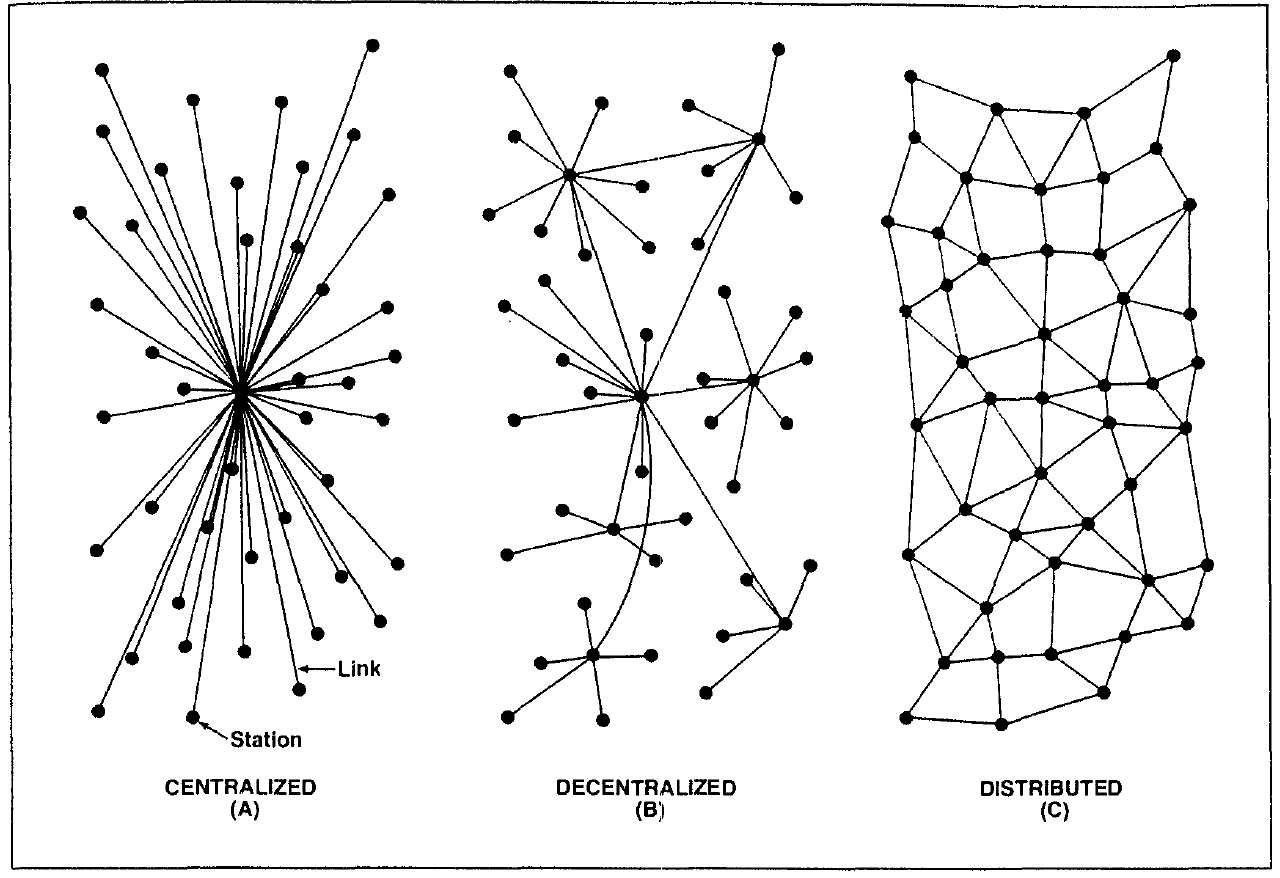
\includegraphics[width=0.8\textwidth]{networks}
  \end{center}
\end{frame}

\begin{frame}
  \frametitle{Peer-to-Peer Networks 2/2}
  \begin{itemize}
  \item In \textbf{centralized} applications, successful attack on the
    \textbf{server} disables the whole application.
  \item In \textbf{decentralized} applications, successful attack on a
    \textbf{hub} results in a temporary network partition, but the application
    remains operational.
  \item In \textbf{peer-to-peer} applications, successful attack on a
    \textbf{peer} has no effect on the network \textit{if the network is big
      enough}.
  \item Example: \textbf{Napster} and \textbf{BitTorrent}.
  \end{itemize}
\end{frame}

\begin{frame}
  \frametitle{Bitcoin Network 2/3}
  \begin{itemize}
  \item \textbf{Bitcoin Network} is a \textbf{peer-to-peer} network that
    consists on \textbf{Bitcoin nodes} that propagate blocks and transactions
    via the \textbf{gossip protocol} and validate them according to
    \textbf{consensus rules}.
  \item According to \textbf{bitnodes.io}, Bitcoin network has approximately
    \textbf{10,000} \textit{listening} (i.e. publicly visible) nodes, but the
    total number of \textbf{full} nodes (i.e. nodes that perform validation of
    chain data) is around \textbf{100,000} nodes.
  \item As of today, 49.5\% of all nodes run the most recent software (Bitcoin
    Core v0.20.1 and v0.21.0).
  \end{itemize}
\end{frame}

\begin{frame}
  \frametitle{Bitcoin Network 3/3}
  \begin{itemize}
  \item As of today, 49.5\% of all nodes run the most recent software (Bitcoin
    Core v0.20.1 and v0.21.0).
  \end{itemize}
  \begin{center}
    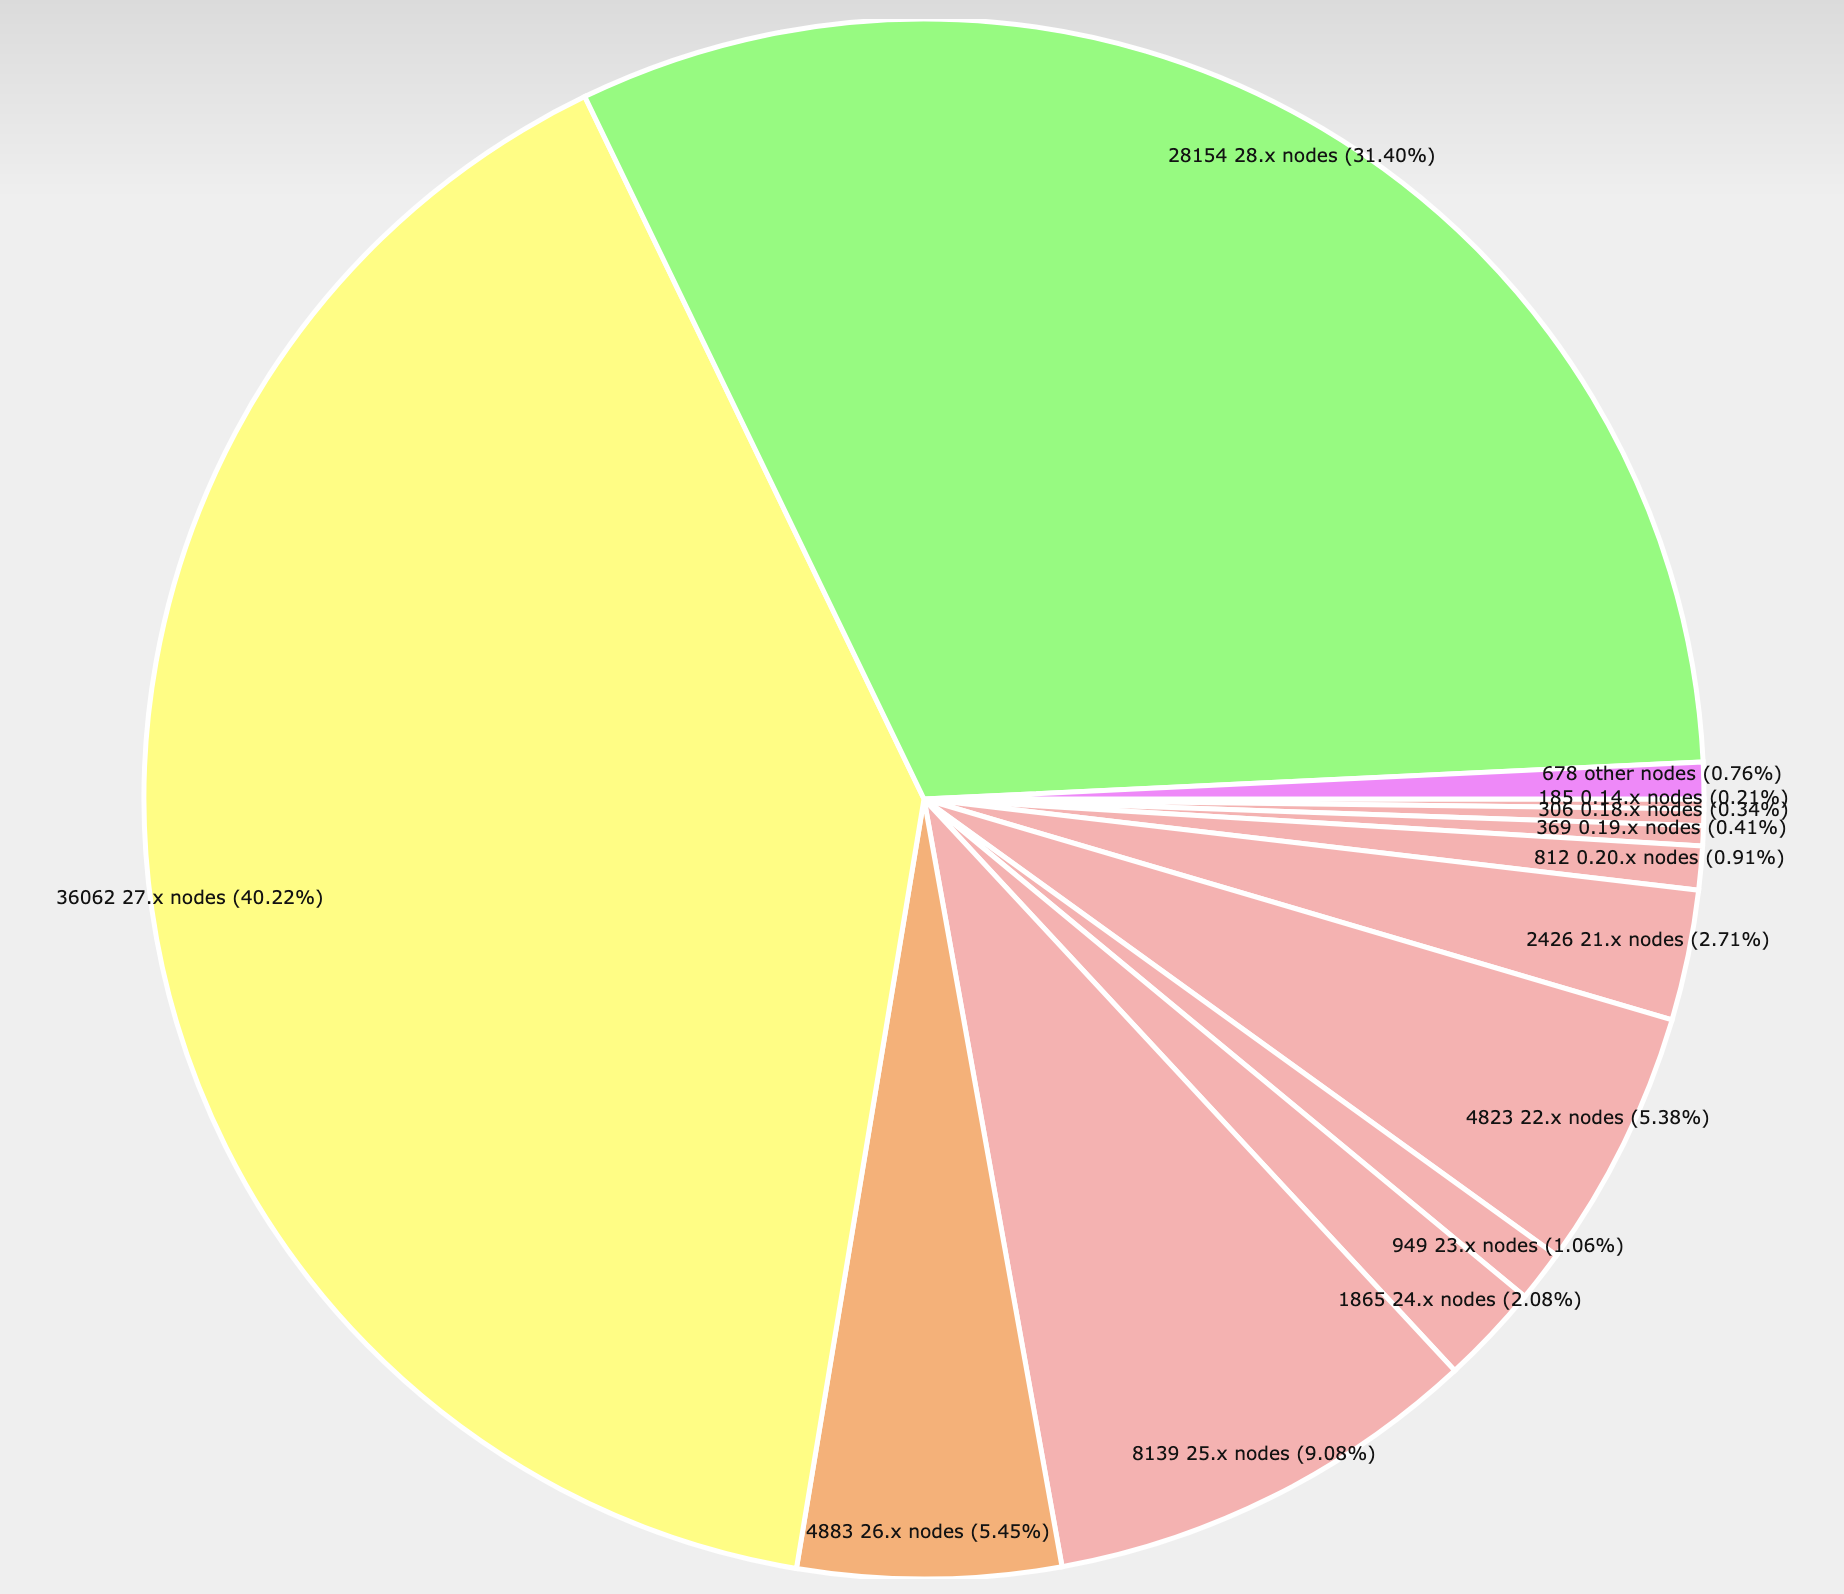
\includegraphics[width=0.7\textwidth]{nodes}
  \end{center}
\end{frame}

\begin{frame}
  \frametitle{Gossip Protocol}
  \begin{itemize}
  \item \textbf{Gossip protocol} (a.k.a. \textbf{epidemic protocol}) is a
    process of peer-to-peer communication that is based on the way
    \textit{epidemics} spread - nodes receive information from one of their
    neighbours and pass it on to all other neighbours.
  \item \textbf{Bitcoin gossip protocol} is a gossip protocol for propagating
    new blocks and transactions as well as providing old blocks from storage to
    new peers on-demand.
  \end{itemize}
  \begin{center}
    \transduration<0-6>{0}
    \multiinclude[<+->][format=png, graphics={width=0.5\textwidth}]{gossip}
  \end{center}
\end{frame}

\begin{frame}
  \frametitle{Bitcoin Network Node}
  \begin{itemize}
  \item \textbf{Bitcoin node} is a member of Bitcoin network, a piece of
    software that executes the gossip protocol and validates the blocks and
    transactions.
  \item A newly started Bitcoin node:
    \begin{itemize}
    \item initializes the connections to several nodes via DNS seeds,
    \item performs \textbf{initial block download} (\textbf{IBD}),
    \item builds necessary indices (UTXO set),
    \item starts listening for new blocks and transactions,
    \item when a new block or transaction is received, node accepts and
      broadcasts it to its peers if is valid, and rejects it otherwise.
    \end{itemize}
  \end{itemize}
\end{frame}

\begin{frame}
  \frametitle{Chain Reorganisation}
  \begin{itemize}
  \item When a new block is received that does not belong to the current chain,
    node attempts to reconnect it to the chain be finding the \textbf{fork
      point}.
  \item Once the block is reconnected, \textbf{the chain that took more energy
      to build} (has the most cumulative \textbf{chainwork}) is chosen as the
    valid chain.
  \item \textbf{Chainwork} is the total number of hashes that are expected to
    have been necessary to produce the current chain.
  \item During IBD, \textbf{headers-first mode} makes this efficient.
  \end{itemize}
\end{frame}

\begin{frame}
  \frametitle{Mempool}
  \begin{itemize}
  \item \textbf{Mempool} is an in-memory data structure that contains all known
    valid transactions that have not been included in any block yet.
  \item Nodes maintain a combined UTXO set that consists of all UTXOs in the
    chain and all UTXOs in the mempool.
  \item When node receives a valid transaction, it adds it to the mempool.
  \item When node receives a new block, it removes all transactions in that
    block from the mempool.
  \item When a node receives a new transaction that conflicts with a transaction
    in its mempool, it rejects the new transaction (except for
    \textbf{replace-by-fee} (\textbf{RBF}) transactions).
  \end{itemize}
\end{frame}

\begin{frame}
  \frametitle{Mining}
  \begin{itemize}
  \item \textbf{Miner nodes} are regular nodes that maintain the mempool and use
    it to build the new blocks.
  \item Miner node sorts mempool by transaction fee and selects ~2000
    transactions to build a new block.
  \item Once a new block is build, miner node passes the block \textbf{template}
    to the mining hardware that starts computing proof-of-work by brute-forcing
    a $SHA256d(block)$ (i.e. $SHA256(SHA256(block))$) value that meets the
    target value.
  \item Once the block is mined (proof-of-work solution is found), the node
    broadcasts it to the network via the gossip protocol.
  \item If another miner mines a different block around the same time, network
    eventually resolves the conflict by selecting the chain with the most work
    (reorg).
  \end{itemize}
\end{frame}

\begin{frame}
  \frametitle{Transaction Lifecycle 1/2}
  \begin{itemize}
  \item Bitcoin transaction destroys a subset of chain/mempool UTXOs and creates
    a set of new mempool ones.
  \item Once signed, transaction is propagated via gossip protocol to all nodes
    on the network, including miner nodes.
  \item Miner nodes see the new transaction and include it in the next block
    template if the transaction fee meets the necessary threshold.
  \item If transaction fee is lower than the threshold for the next block, it
    remains in the mempool until all the higher-fee transactions are confirmed.
  \end{itemize}
\end{frame}

\begin{frame}
  \frametitle{Transaction Lifecycle 2/2}
  \begin{itemize}
  \item While in the mempool, transaction be ``bumped'' higher in the mempool
    using the following
    \begin{itemize}
    \item \textbf{replace-by-fee} (\textbf{RBF}),
    \item \textbf{Child Pays For Parent} (\textbf{CPFP}).
    \end{itemize}
  \item Once the block with the transaction is mined and propagated through the
    network, on every node in the network that saw the new block
    \begin{itemize}
    \item transaction is removed from the mempool,
    \item transaction is applied to the UTXO set (UTXOs that are destroyed by
      the transaction are removed from the UTXO set and UTXOs that are created
      by the transaction are added to the UTXO set).
    \end{itemize}
  \end{itemize}
\end{frame}

\begin{frame}
  \frametitle{The End}
  \begin{center}
    Thank you!
  \end{center}
\end{frame}

\end{document}

%%% Local Variables:
%%% mode: latex
%%% TeX-master: t
%%% End:
